\documentclass[12pt,letterpaper]{article}
\usepackage[utf8]{inputenc}
\usepackage[spanish]{babel}
\usepackage{graphicx}
\usepackage{tabularx}
\usepackage{multirow}
\usepackage{float}
\usepackage{hyperref}
\usepackage{enumerate} 

\begin{document}
\begin{center}
{\Large \textbf{Métodos Computacionales - Taller 5}}\\
\vspace{0.3cm}
\textbf{Julián Leandro Rodríguez Cardona - 201416065}\\ \vspace{0.3cm}
\end{center}

\section*{Métodos de Monte Carlo}

Este taller consistía de dos ejercicios. En el primero nos suministran datos de la ubicación de las moléculas que conforman las paredes de un canal iónico y el objetivo es hallar el poro dentro del canal; en este caso, ya que es en dos dimensiones, debemos hallar el círculo con mayor radio que quepa dentro del canal sin tocar las paredes del mismo. Para realizar lo anterior, implementamos el método de Cadenas de Markov de Monte Carlo (Markov Chain - Monte Carlo) y lo hacemos para dos canales distintos dados por dos archivos.

En el segundo ejercicio nos suministran datos observados para el comportamiento de la carga de un condensador en un circuito RC y el objetivo es determinar el valor de la resistencia (R) y el del capacitor (C) que mejor se ajusten. Para esto, implementamos un método de estimación Bayesiana de parámetros con Monte Carlo, utilizando el modelo de la función de carga de un condensador en un circuito RC:

$$ Q(t) = V_0 C \left( 1- e^{-t/RC} \right) $$

A continuación se presentan los resultados obtenidos.

\section{Canales iónicos}

\subsection{Resultados para el archivo ''Canal\_ionico.txt". }
\begin{figure}[H]
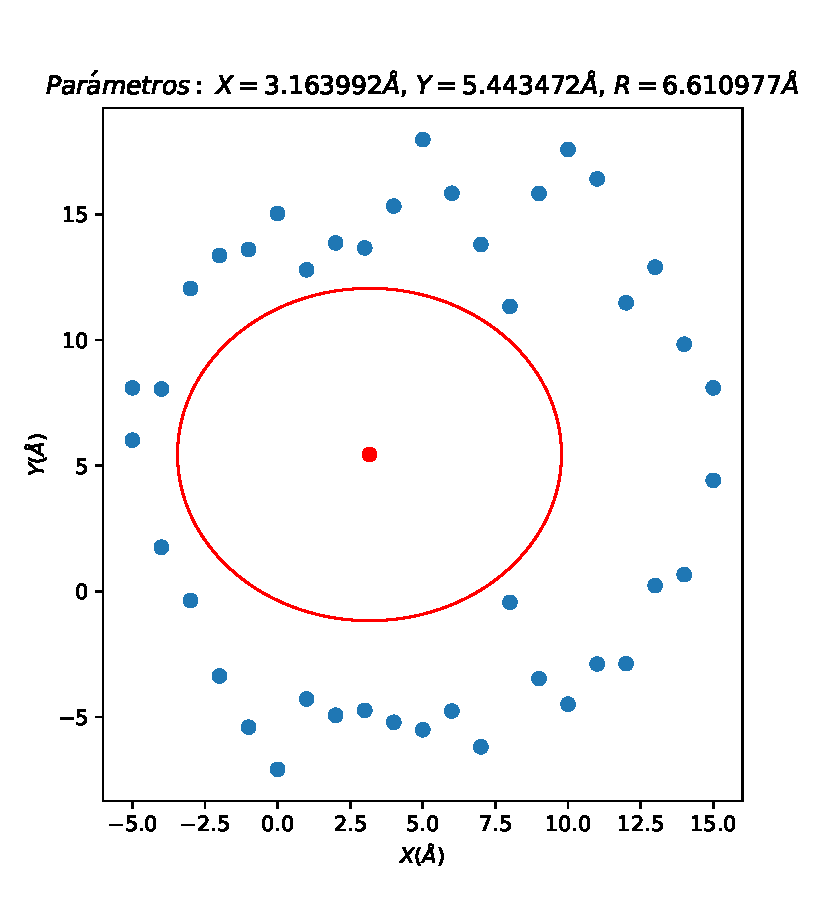
\includegraphics{canal.pdf}
\caption{Circulo de máximo radio en el canal del archivo ''Canal\_ionico.txt".}
\centering
\end{figure}

\begin{figure}[H]
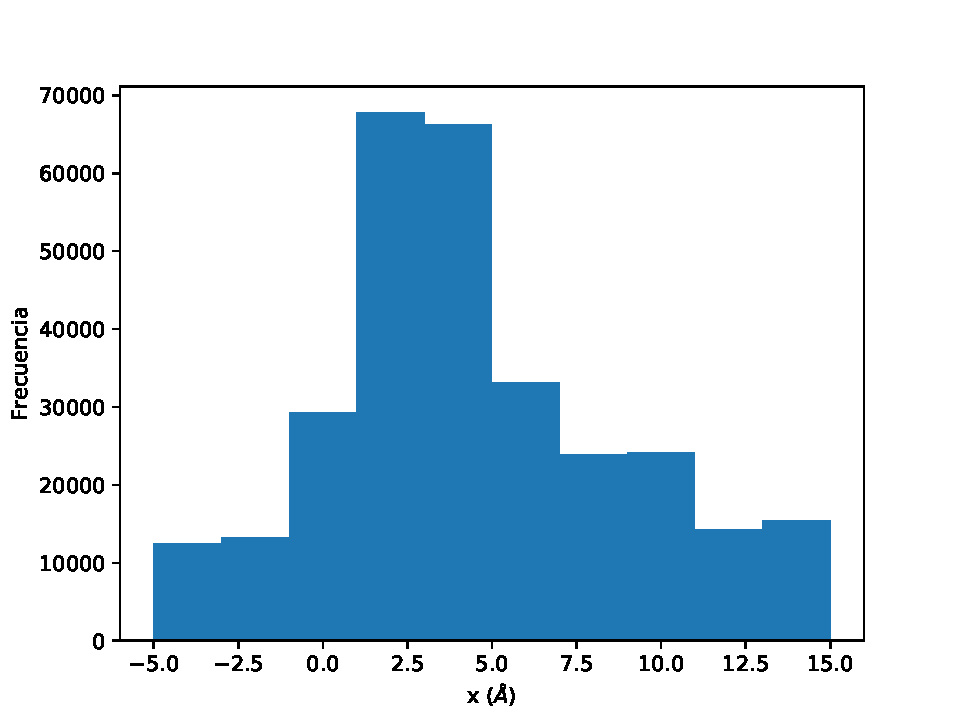
\includegraphics{x_hist.pdf}
\caption{Histograma de la coordenada x.}
\centering
\end{figure}

\begin{figure}[H]
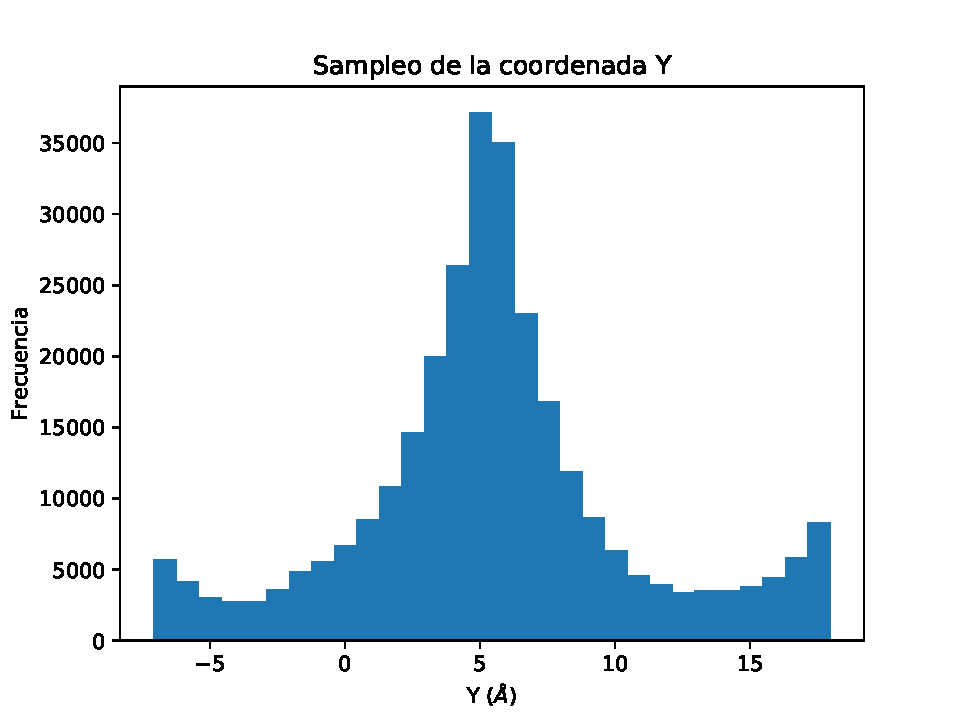
\includegraphics{y_hist.pdf}
\caption{Histograma de la coordenada y.}
\centering
\end{figure}

\subsection{Resultados para el archivo ''Canal\_ionico1.txt". }

\begin{figure}[H]
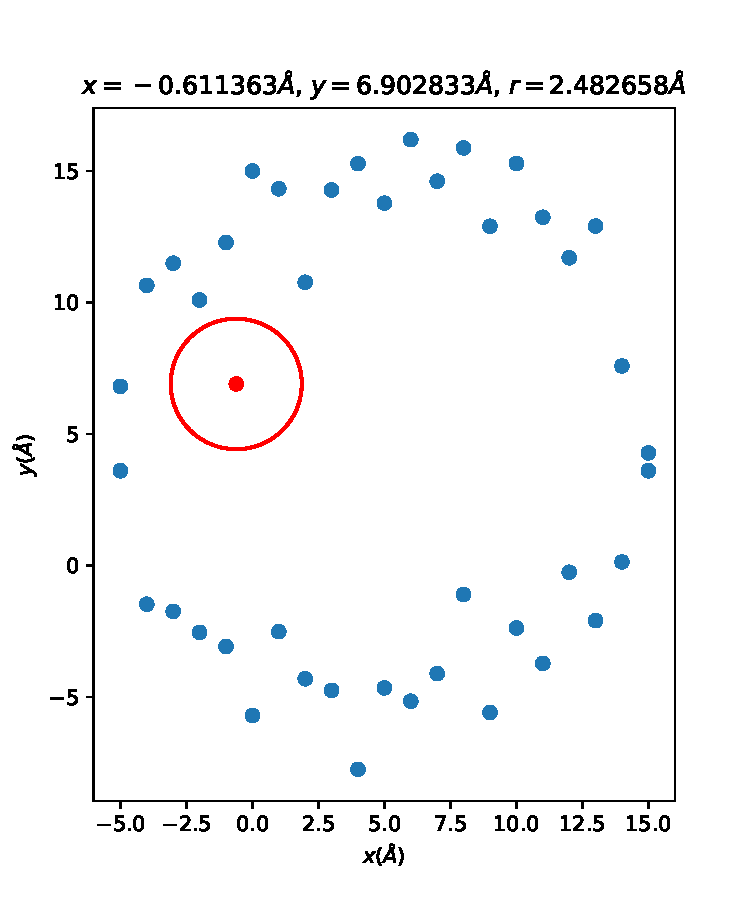
\includegraphics{canal1.pdf}
\caption{Circulo de máximo radio en el canal del archivo ''Canal\_ionico1.txt".}
\centering
\end{figure}

\begin{figure}[H]
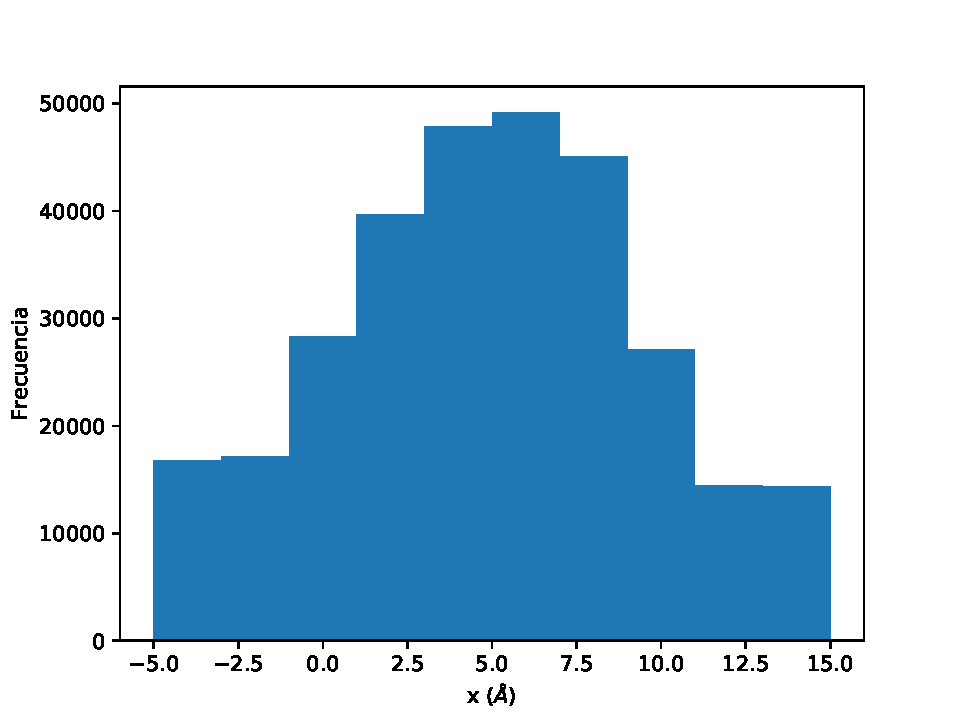
\includegraphics{x1_hist.pdf}
\caption{Histograma de la coordenada x.}
\centering
\end{figure}

\begin{figure}[H]
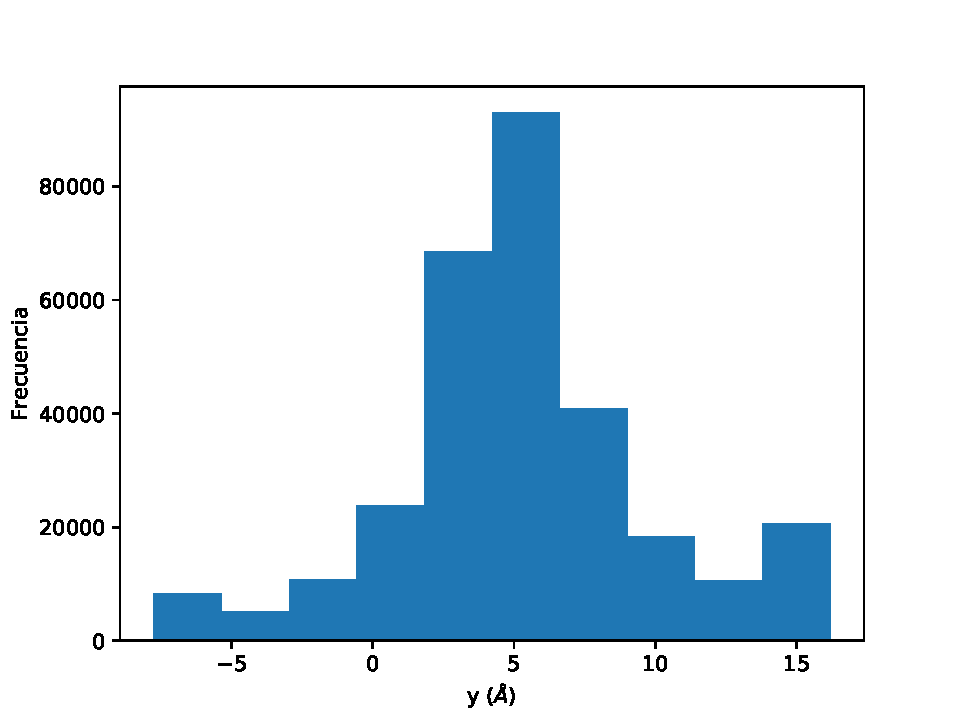
\includegraphics{y1_hist.pdf}
\caption{Histograma de la coordenada y.}
\centering
\end{figure}

\section{Circuito RC}

\subsection{Resistencia}

\begin{figure}[H]
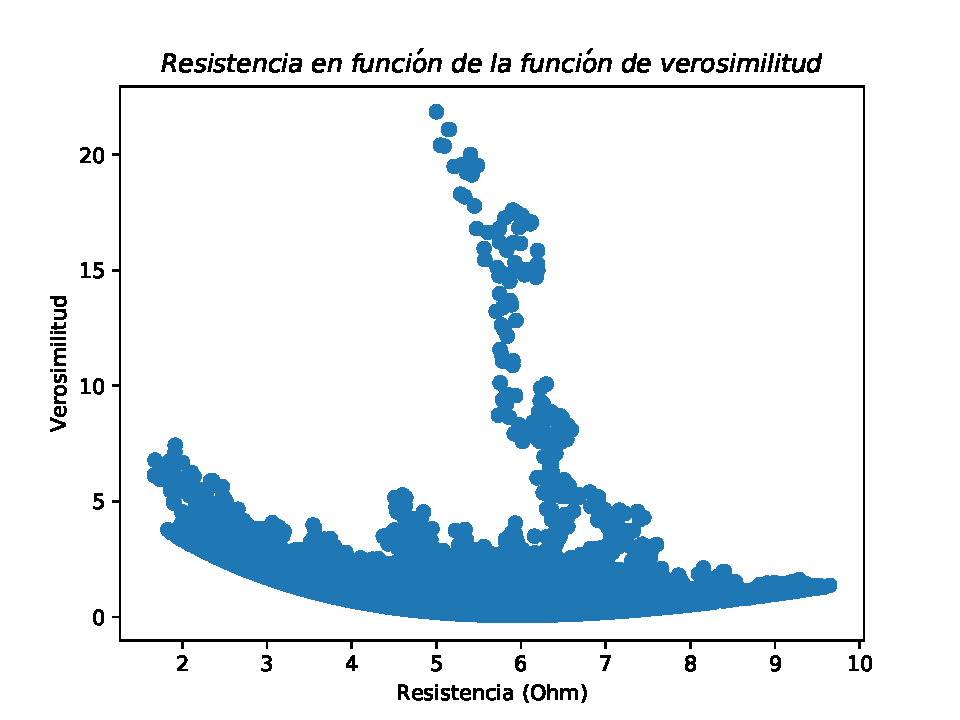
\includegraphics{r_verosimilitud.pdf}
\caption{Valores de la resistencia en función de la función de verosimilitud.}
\centering
\end{figure}

\begin{figure}[H]
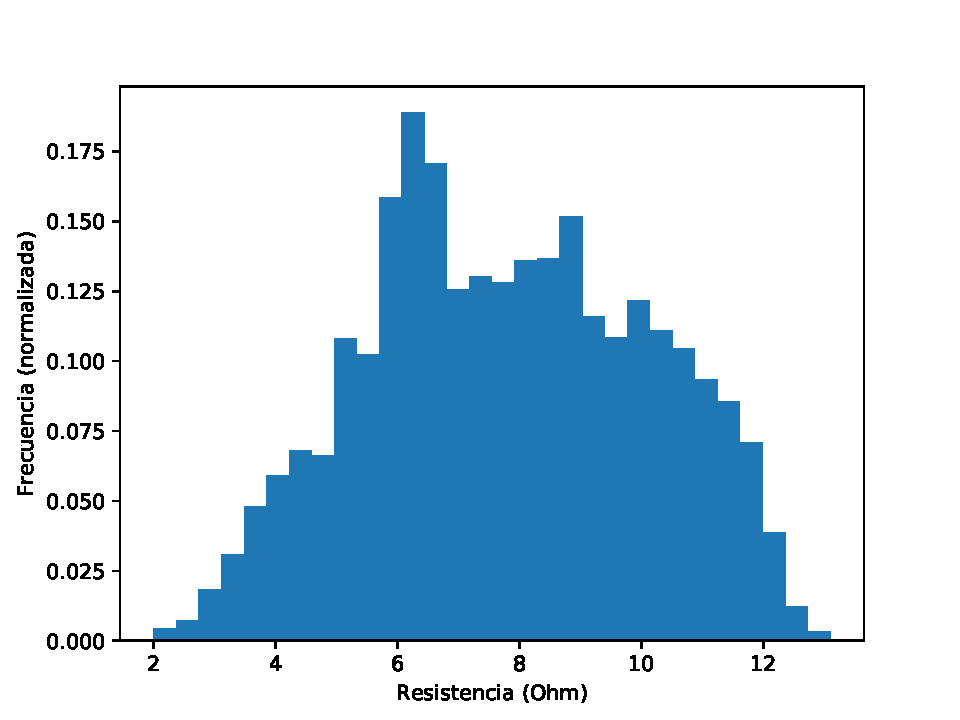
\includegraphics{r_hist.pdf}
\caption{Sampleo del valor de la resistencia.}
\centering
\end{figure}

\subsection{Capacitancia}

\begin{figure}[H]
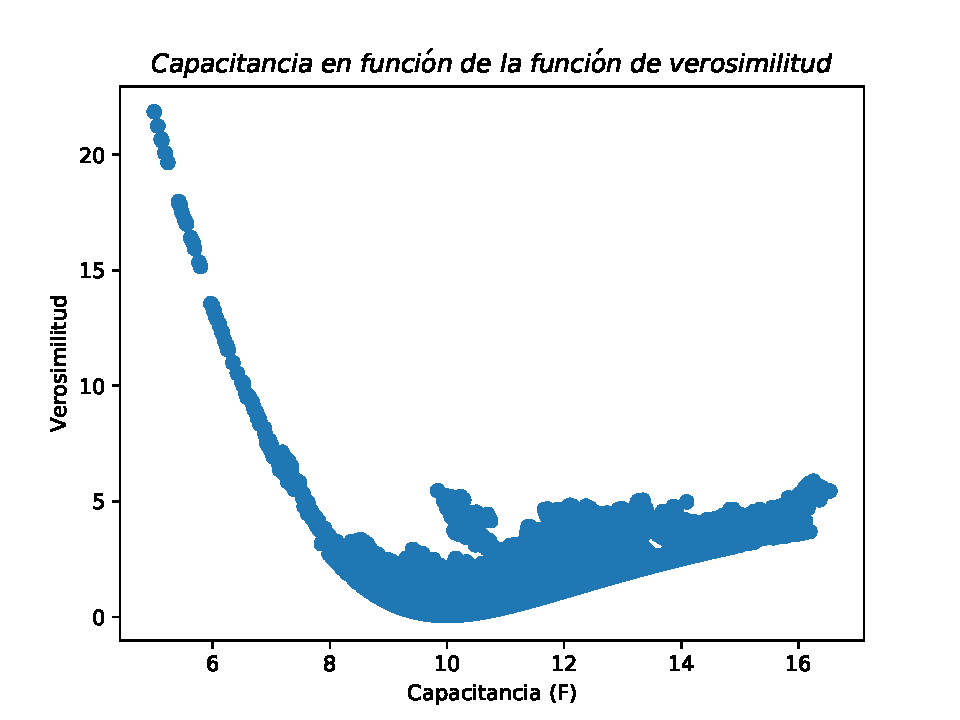
\includegraphics{c_verosimilitud.pdf}
\caption{Valores de la capacitancia en función de la función de verosimilitud.}
\centering
\end{figure}

\begin{figure}[H]
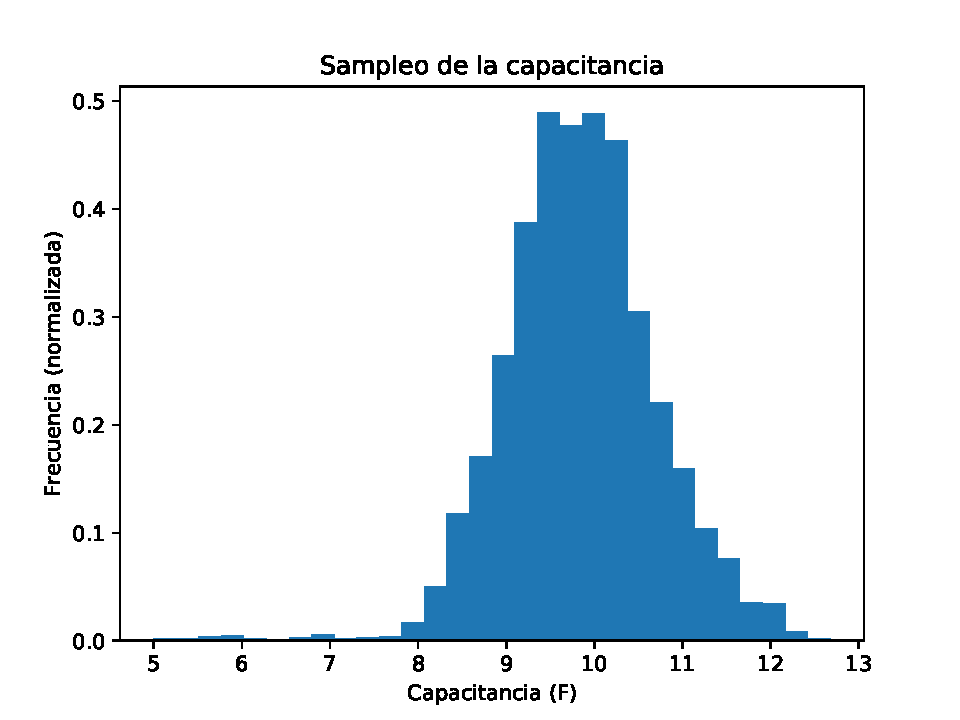
\includegraphics{c_hist.pdf}
\caption{Sampleo del valor de la capacitancia.}
\centering
\end{figure}

\subsection{Carga en función del tiempo}
\begin{figure}[H]
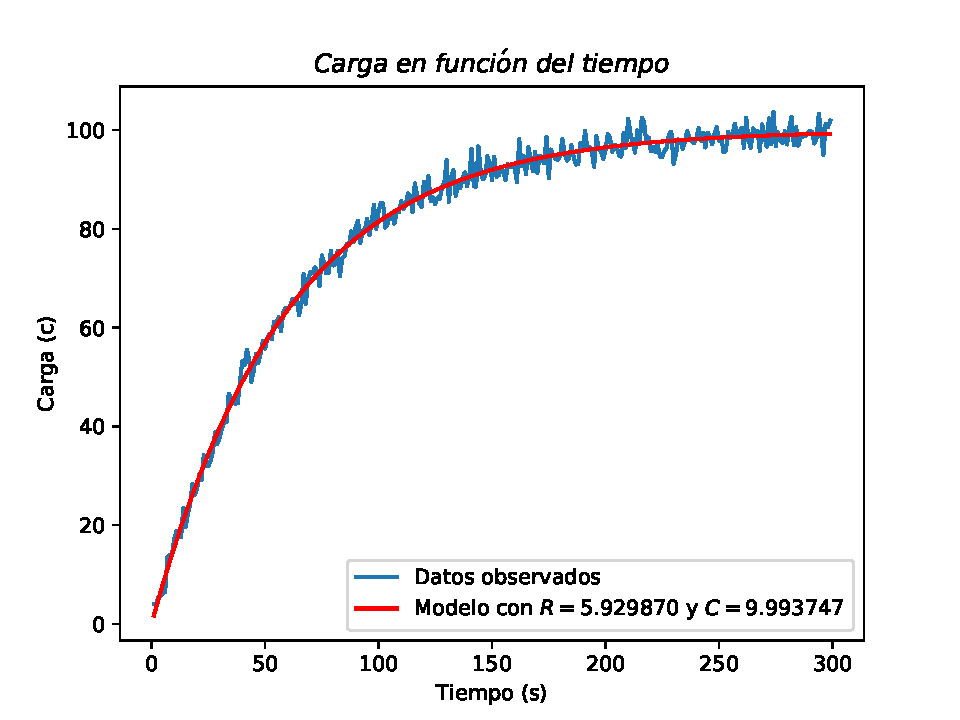
\includegraphics{carga.pdf}
\caption{Datos obsevados y modelo con datos ideales obtenido para la carga del condensador en función del tiempo.}
\centering
\end{figure}

\vspace{0.3cm}


\end{document}
